\section{Preliminaries}

\subsection{Allocations}
\begin{frame}{Allocations}
	Setting:
	\begin{itemize}
		\item
		recipients: set \(\agents\) of \(n\) agents

		\item
		goods: set \(\goods\) of \(m\) items
		\begin{itemize}
			\item
			unsharable

			\item
			indivisible
		\end{itemize}
	\end{itemize}
	\begin{definition}[1]
		An \emph{allocation} is a tuple
		\(\alloc[][] = (\alloc)_{i \in \agents}\)
		of bundles \(\alloc \subset \goods\) such that each item is element of precisely one bundle.

		Item \(j\) is \emph{assigned} to agent \(i\) if \(j \in \alloc\).
	\end{definition}

	But how to measure its efficiency and fairness?
\end{frame}





\subsection{Valuation Functions}
\begin{frame}{Valuation Functions}{}
	Requirements:
	\vspace{-0.5ex}
	\begin{itemize}
		\item
		monotonically non-decreasing: \(\valuations[\genericset[1]] \le \valuations[\genericset[2]]\) \quad \(\forall \genericset[1] \subset \genericset[2] \subset \goods\)

		\item
		normalised: \(\valuations[\emptyset] = 0\)

		\item
		non-negative: \(\valuations[\genericset] \ge 0\) \quad \(\forall \genericset \subset \goods\)
	\end{itemize}

	Types:
	\vspace{-0.5ex}
	\begin{itemize}
		\item
		additive: \(\valuations[\genericset] \coloneq \sum_{\genericitem \in \genericset} \valuations[ \hairspace \genericitem ]\) \quad \(\forall \genericset \subset \goods\)

		\item
		submodular: \(\valuations[\genericset[1] \given \genericset[2]] \coloneq \valuations[\genericset[1] \cup \genericset[2]] - \valuations[\genericset[2]]\) \quad \(\forall \genericset[1], \genericset[2] \subset \goods\) with \(\genericset[1], \genericset[2]\) disjoint
		\begin{itemize}
			\item
			more general (encompasses additivity)

			\item
			diminishing returns
		\end{itemize}
	\end{itemize}

	\begin{center}
		
\includegraphics[height=2cm]{img/additive}
		\hfil
		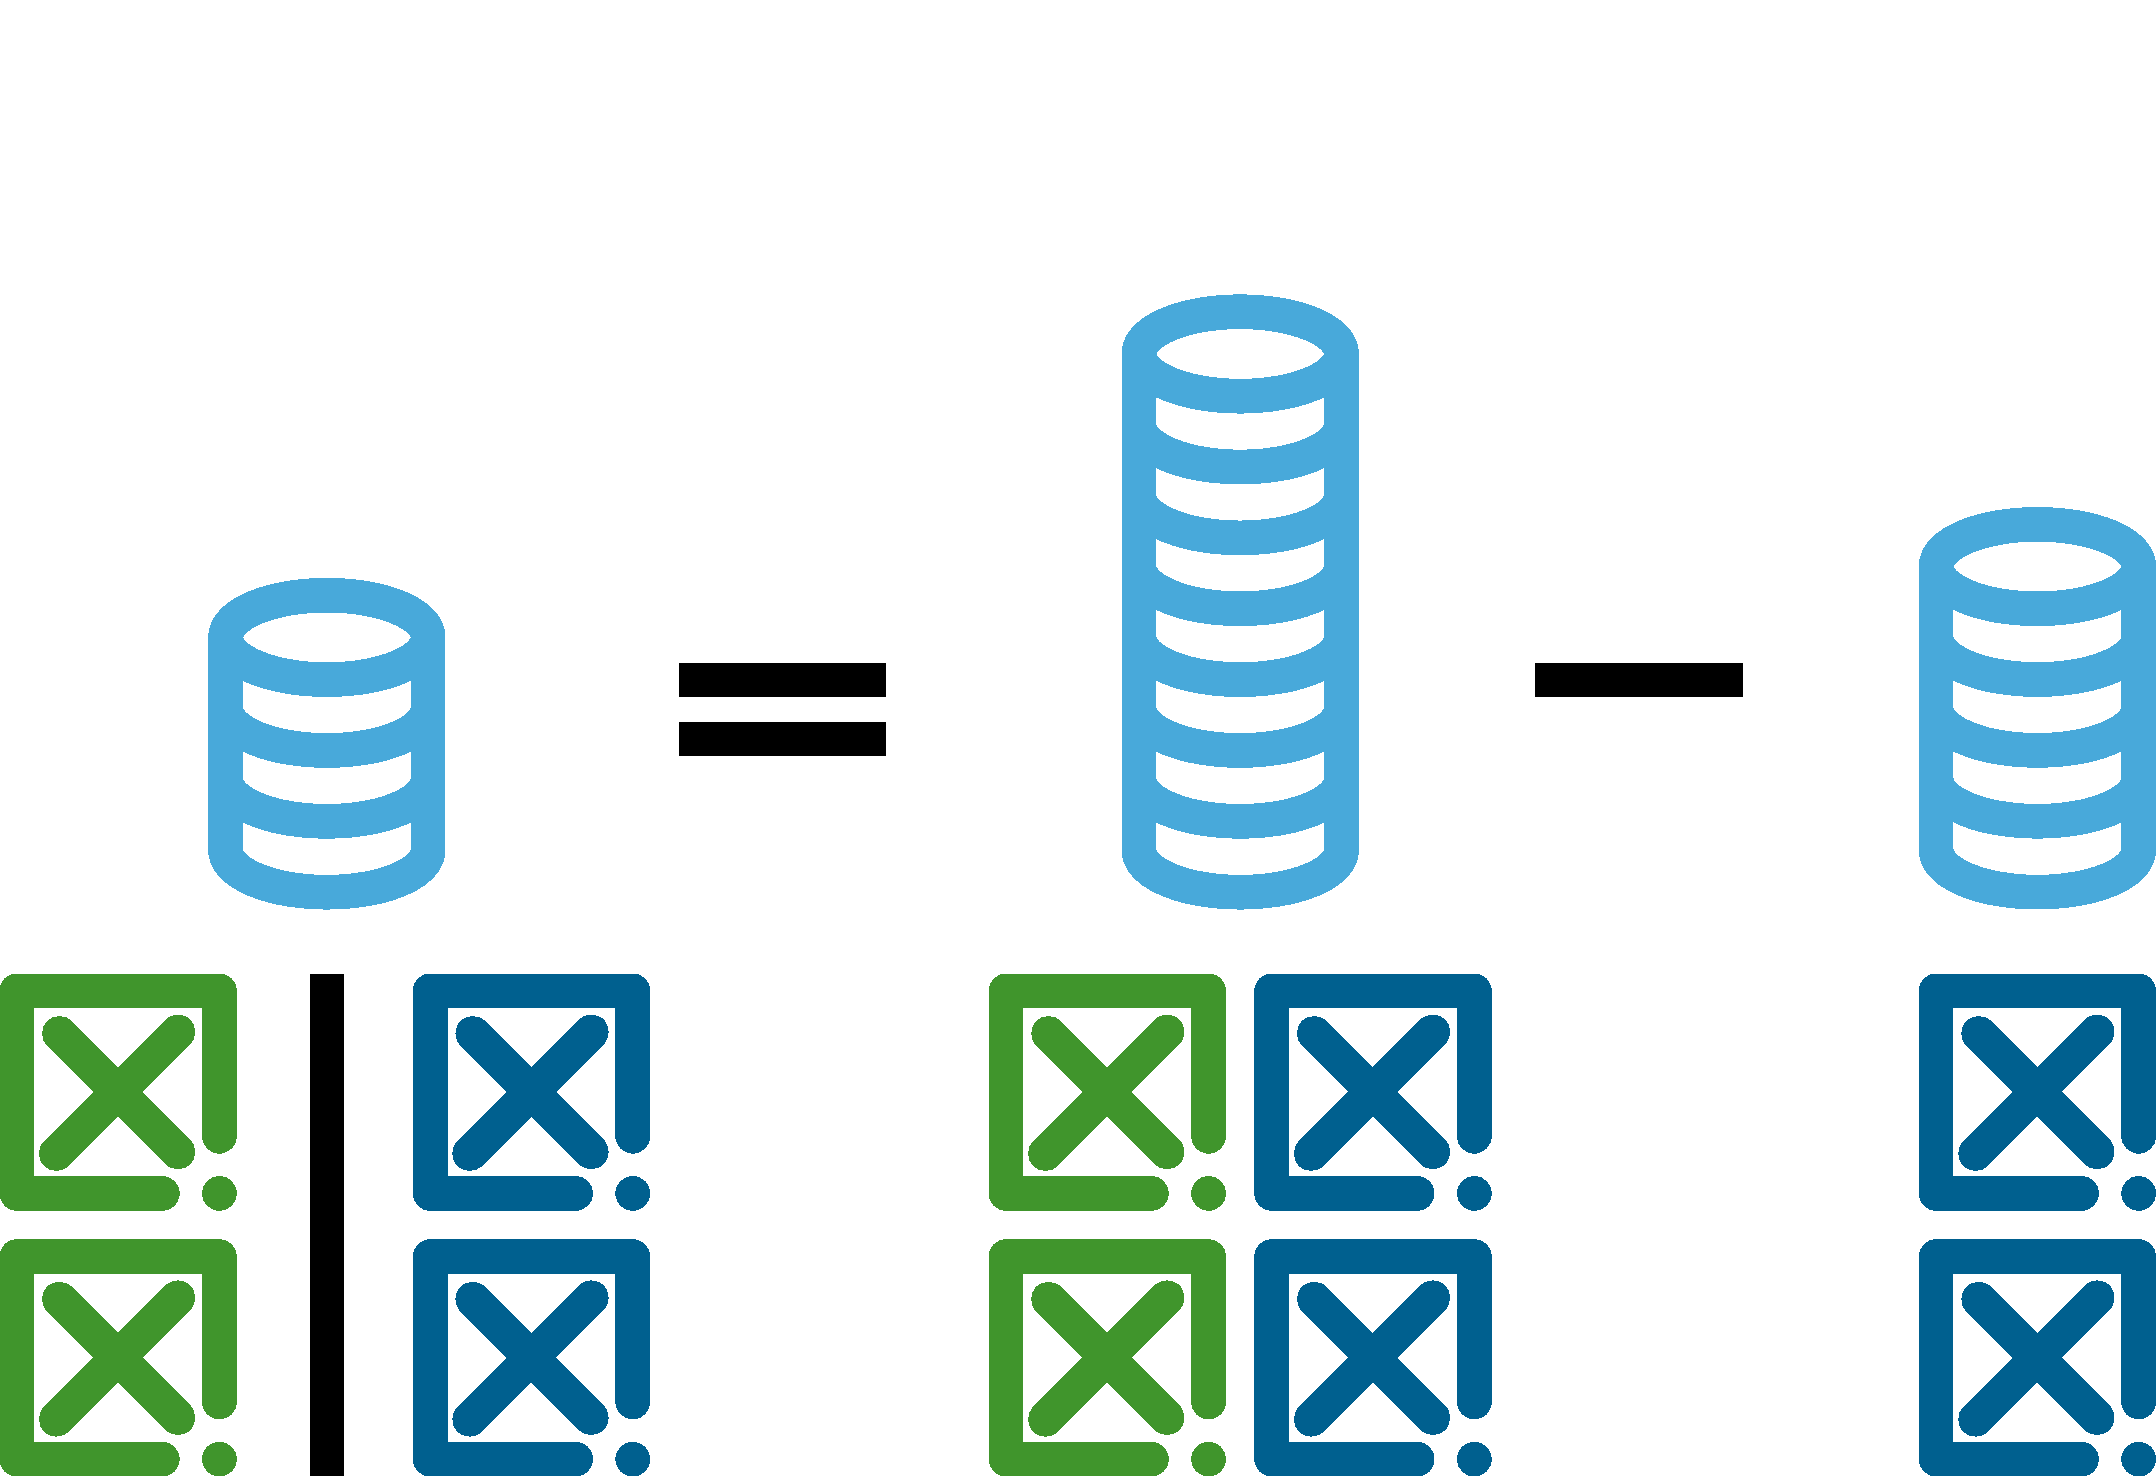
\includegraphics[height=2cm]{img/submodular}
		\hfil
		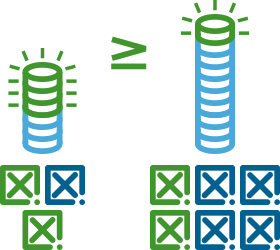
\includegraphics[height=2cm]{img/diminishingreturns}
	\end{center}
\end{frame}





\subsection{Maximum Nash Social Welfare Problem}
\begin{frame}{Asymmetric Maximum Nash Social Welfare Problem}
	\adjustfortopblock
	\begin{problem}[2]
		\begin{equation*}
			\alloc*[][] \overset{!}{=} \smashoperator{\argmax_{\alloc[][] \in \allallocs{\scriptstyle\agents\kern1pt}{\goods}}} \braces{ \NSW(\alloc[][]) }
			\quad\text{with~}
			\NSW(\alloc[][]) \coloneq \paren[\Big]{ \smashoperator{\prod_{i \in \agents}} \valuations[\alloc]^{\,\textstyle\weight} }{}^{\textstyle 1 / \sum_{i \in \agents} \weight}
		\end{equation*}
		\begin{itemize}
			\item
			\(\allallocs{\agents\kern1pt}{\goods}\): all possible allocations

			\item
			\(\weight\): agent weight
		\end{itemize}
	\end{problem}
	The NSW strikes a middle ground between efficiency and fairness!

	\medskip

	\begin{minipage}{0.6\textwidth}
		\begin{alertblock}{Challenge}
			Algorithm with approximation factor \emph{independent from \(m\)}!
		\end{alertblock}
	\end{minipage}

	\beamerimage at (13cm, 0.25cm) {
\includegraphics[height=3cm]{img/nvsm}};
\end{frame}